\documentclass[10pt]{article}
\usepackage{tikz}
\usetikzlibrary{shapes.misc}
\usepackage[margin=0cm]{geometry}
\pagestyle{empty}
\tikzstyle{every node}=[cross out, draw, red]

\begin{document}

\vspace*{\fill}
\begin{center}
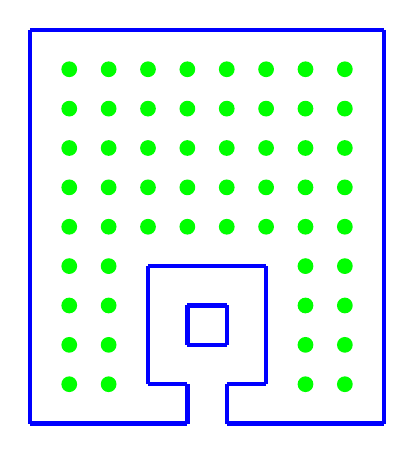
\begin{tikzpicture}[x=0.5cm, y=-0.5cm, ultra thick, blue]
% Walls
    \draw (0,0) -- (9,0);
    \draw (3,6) -- (6,6);
    \draw (4,7) -- (5,7);
    \draw (4,8) -- (5,8);
    \draw (3,9) -- (4,9);
    \draw (5,9) -- (6,9);
    \draw (0,10) -- (4,10);
    \draw (5,10) -- (9,10);
    \draw (0,0) -- (0,10);
    \draw (3,6) -- (3,9);
    \draw (4,7) -- (4,8);
    \draw (4,9) -- (4,10);
    \draw (5,7) -- (5,8);
    \draw (5,9) -- (5,10);
    \draw (6,6) -- (6,9);
    \draw (9,0) -- (9,10);
% Pillars
    \fill[green] (1,1) circle(0.2);
    \fill[green] (2,1) circle(0.2);
    \fill[green] (3,1) circle(0.2);
    \fill[green] (4,1) circle(0.2);
    \fill[green] (5,1) circle(0.2);
    \fill[green] (6,1) circle(0.2);
    \fill[green] (7,1) circle(0.2);
    \fill[green] (8,1) circle(0.2);
    \fill[green] (1,2) circle(0.2);
    \fill[green] (2,2) circle(0.2);
    \fill[green] (3,2) circle(0.2);
    \fill[green] (4,2) circle(0.2);
    \fill[green] (5,2) circle(0.2);
    \fill[green] (6,2) circle(0.2);
    \fill[green] (7,2) circle(0.2);
    \fill[green] (8,2) circle(0.2);
    \fill[green] (1,3) circle(0.2);
    \fill[green] (2,3) circle(0.2);
    \fill[green] (3,3) circle(0.2);
    \fill[green] (4,3) circle(0.2);
    \fill[green] (5,3) circle(0.2);
    \fill[green] (6,3) circle(0.2);
    \fill[green] (7,3) circle(0.2);
    \fill[green] (8,3) circle(0.2);
    \fill[green] (1,4) circle(0.2);
    \fill[green] (2,4) circle(0.2);
    \fill[green] (3,4) circle(0.2);
    \fill[green] (4,4) circle(0.2);
    \fill[green] (5,4) circle(0.2);
    \fill[green] (6,4) circle(0.2);
    \fill[green] (7,4) circle(0.2);
    \fill[green] (8,4) circle(0.2);
    \fill[green] (1,5) circle(0.2);
    \fill[green] (2,5) circle(0.2);
    \fill[green] (3,5) circle(0.2);
    \fill[green] (4,5) circle(0.2);
    \fill[green] (5,5) circle(0.2);
    \fill[green] (6,5) circle(0.2);
    \fill[green] (7,5) circle(0.2);
    \fill[green] (8,5) circle(0.2);
    \fill[green] (1,6) circle(0.2);
    \fill[green] (2,6) circle(0.2);
    \fill[green] (7,6) circle(0.2);
    \fill[green] (8,6) circle(0.2);
    \fill[green] (1,7) circle(0.2);
    \fill[green] (2,7) circle(0.2);
    \fill[green] (7,7) circle(0.2);
    \fill[green] (8,7) circle(0.2);
    \fill[green] (1,8) circle(0.2);
    \fill[green] (2,8) circle(0.2);
    \fill[green] (7,8) circle(0.2);
    \fill[green] (8,8) circle(0.2);
    \fill[green] (1,9) circle(0.2);
    \fill[green] (2,9) circle(0.2);
    \fill[green] (7,9) circle(0.2);
    \fill[green] (8,9) circle(0.2);
% Inner points in accessible cul-de-sacs
% Entry-exit paths without intersections
\end{tikzpicture}
\end{center}
\vspace*{\fill}

\end{document}
